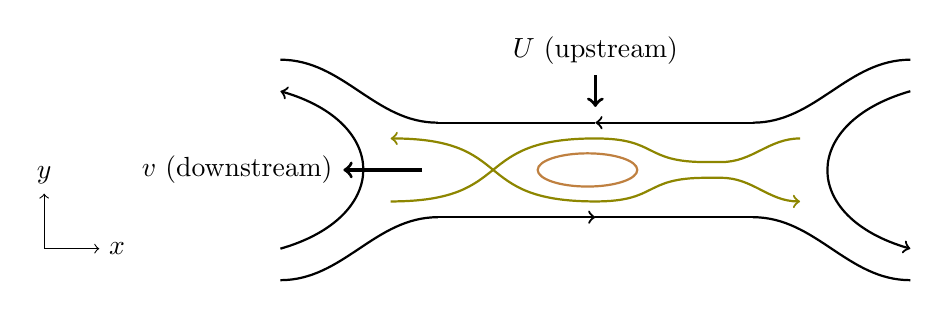
\begin{tikzpicture}

% _____ Reference frame
\def\RefFrameX{-7.0}
\def\RefFrameY{-1.0}
\def\RefFrameLen{0.7}

\draw[->] (\RefFrameX, \RefFrameY) -- (\RefFrameX+\RefFrameLen, \RefFrameY) node[right]{$x$} ;
\draw[->] (\RefFrameX, \RefFrameY) -- (\RefFrameX, \RefFrameY+\RefFrameLen) node[above]{$y$} ;

% _____ Diffusion region 
\def\DiffusionLen{2.0}
\def\DiffusionWidth{0.4}
\def\DiffusionParam{0.8}

% \fill[gray!40] (-\DiffusionLen, -\DiffusionWidth) rectangle (\DiffusionLen, \DiffusionWidth);
% \node at (0.0, -\DiffusionWidth) {$L$};
% \node at (\DiffusionLen, 0) {$\delta_{\mathrm{SP}}$};

% _____ Magnetic field lines
\def\BLineGap{0.2}
\def\BLineX{2.0}
\def\BLineY{1.0}

\draw[thick, <-] (0, \DiffusionWidth+\BLineGap) -- (\DiffusionLen, \DiffusionWidth+\BLineGap);
\draw[thick] (\DiffusionLen, \DiffusionWidth+\BLineGap)
    .. controls +(\DiffusionParam, 0) and +(-\DiffusionParam, 0)
    .. (\DiffusionLen+\BLineX, \DiffusionWidth+\BLineY);

\draw[thick] (0, -\DiffusionWidth-\BLineGap) -- (\DiffusionLen,-\DiffusionWidth-\BLineGap);
\draw[thick] (\DiffusionLen, -\DiffusionWidth-\BLineGap)
    .. controls +(\DiffusionParam, 0) and +(-\DiffusionParam, 0)
    .. (\DiffusionLen+\BLineX, -\DiffusionWidth-\BLineY);


\draw[thick] (0, \DiffusionWidth+\BLineGap) -- (-\DiffusionLen, \DiffusionWidth+\BLineGap);
\draw[thick] (-\DiffusionLen, \DiffusionWidth+\BLineGap)
    .. controls +(-\DiffusionParam, 0) and +(+\DiffusionParam, 0)
    .. (-\DiffusionLen-\BLineX, \DiffusionWidth+\BLineY);

\draw[thick, <-] (0, -\DiffusionWidth-\BLineGap) -- (-\DiffusionLen,-\DiffusionWidth-\BLineGap);
\draw[thick] (-\DiffusionLen, -\DiffusionWidth-\BLineGap)
    .. controls +(-\DiffusionParam, 0) and +(+\DiffusionParam, 0)
    .. (-\DiffusionLen-\BLineX, -\DiffusionWidth-\BLineY);

\def\BCloseX{4.0}
\def\BCloseDy{1.0}
\def\BCloseNode{2.6}
\def\BCloseDeltaNode{0.6}
\draw[thick, ->] (\BCloseX, +\BCloseDy)
    .. controls (\BCloseNode, +\BCloseDeltaNode) and (\BCloseNode, -\BCloseDeltaNode)
    .. (\BCloseX, -\BCloseDy);

\draw[thick, <-] (-\BCloseX, +\BCloseDy)
    .. controls (-\BCloseNode, +\BCloseDeltaNode) and (-\BCloseNode, -\BCloseDeltaNode)
    .. (-\BCloseX, -\BCloseDy);

\def\BPlasmoidX{2.6}
\def\BPlasmoidY{0.4}
\def\BPlasmoidDx{1.6}

\def\BPlasmoidXPrime{1.4}
\def\BPlasmoidDxPrime{0.8}
\def\BPlasmoidDxPrimePrime{0.4}
\def\BPlasmoidDelta{0.2}
\def\BPlasmoidDy{0.1}

\draw[thick, olive] (-\BPlasmoidX, -\BPlasmoidY)
    .. controls +(+\BPlasmoidDx, 0) and +(-\BPlasmoidDx, 0)
    .. (0, +\BPlasmoidY)
    .. controls +(+\BPlasmoidDxPrime, 0) and +(-\BPlasmoidDxPrime, 0)
    .. (+\BPlasmoidXPrime, \BPlasmoidDy) -- (+\BPlasmoidXPrime+\BPlasmoidDelta, \BPlasmoidDy)
    .. controls +(+\BPlasmoidDxPrimePrime, 0) and +(-\BPlasmoidDxPrimePrime, 0)
    .. (+\BPlasmoidX, \BPlasmoidY);

\draw[thick, <->, olive] (-\BPlasmoidX, +\BPlasmoidY)
    .. controls +(+\BPlasmoidDx, 0) and +(-\BPlasmoidDx, 0)
    .. (0, -\BPlasmoidY)
    .. controls +(+\BPlasmoidDxPrime, 0) and +(-\BPlasmoidDxPrime, 0)
    .. (+\BPlasmoidXPrime, -\BPlasmoidDy) -- (+\BPlasmoidXPrime+\BPlasmoidDelta, -\BPlasmoidDy)
    .. controls +(+\BPlasmoidDxPrimePrime, 0) and +(-\BPlasmoidDxPrimePrime, 0)
    .. (+\BPlasmoidX, -\BPlasmoidY);

% \draw[thick, ->, olive] (-\BPlasmoidX, -\BPlasmoidY)
%     .. controls +(+\BPlasmoidDx, 0) and +(-\BPlasmoidDx, 0)
%     .. (0, +\BPlasmoidY)
%     .. controls +(+\BPlasmoidDx, 0) and +(-\BPlasmoidDx, 0)
%     .. (+\BPlasmoidX, -\BPlasmoidY);
% 
% \draw[thick, <-, olive] (-\BPlasmoidX, +\BPlasmoidY)
%     .. controls +(+\BPlasmoidDx, 0) and +(-\BPlasmoidDx, 0)
%     .. (0, -\BPlasmoidY)
%     .. controls +(+\BPlasmoidDx, 0) and +(-\BPlasmoidDx, 0)
%     .. (+\BPlasmoidX, +\BPlasmoidY);

\draw[thick, brown] (-0.1,0) circle [x radius=18pt, y radius=6pt];







% _____ legends
\def\UpstreamU{0.4}
\def\Downstreamv{1.0}

\draw[very thick, <-] (0, \DiffusionWidth+2*\BLineGap) -- (0, \DiffusionWidth+2*\BLineGap+\UpstreamU) node[above]{$U$ (upstream)} ;
\draw[very thick, ->] (-\DiffusionLen-\BLineGap, 0) -- (-\DiffusionLen-\BLineGap-\Downstreamv, 0) node[left]{$v$ (downstream)} ;

% \node at (0.0, 0.0) {$\eta \mu_0 J > U B_0$};
% \node at (0.0, 0.0) {$E_z^{\mathrm{diff}} > E_z^{\mathrm{ideal}}$};

\end{tikzpicture}
